\begin{abstract}
Crowdsourced cultural maps can turn documentation geography into an artist identity label and then reuse that label to measure international activity. We audit this boundary using the published street-art origin rule and 48,690 markers in six October 2026 Street Art Cities exports. Among 3,051 qualifying single-artist profiles, geography-derived anchors classify 94.1\% of 30,696 documented works as domestic. This statistic describes concentration around an inferred anchor, rather than independently establishing biographical origin. In a conservative comparison, 196 of 933 artists have anchors inconsistent with their recorded nationality tags; 172 of these disagreements involve countries outside the export panel. Removing each artist's largest collector reassigns 38 anchors, compared with a mean of 8.5 under equal-size random marker deletion. We derive exact documentation-completion costs and sharp fixed-cohort sensitivity envelopes, including joint witnesses for destination-ranking reversals. Fourteen additional documented works suffice to reverse the Portugal--Belgium ordering; 352 suffice to reverse the Netherlands--Spain ordering. These are conditional robustness results, not estimates of unseen production. A four-country monthly replay finds no resolved anchor changes, demonstrating that short-term stability need not establish construct validity. The contribution is a reproducible audit of how coverage becomes cultural identity, with an implementable reporting discipline separating biographical evidence, documented anchors, and support-dependent uncertainty.
\end{abstract}
\ccsdesc[300]{Information systems~Data mining}
\keywords{cultural data, street art, construct validity, geographic coverage, algorithmic accountability, sensitivity analysis}
\maketitle

\section{Introduction}
A mural has a location. Its artist may have a birthplace, several national affiliations, a changing place of residence, and an international career. A cultural platform records only some of that career, through contributors whose attention is unevenly distributed. These quantities can nevertheless become a single country label in a data pipeline. Once a label is called an artist's origin, comparing it with mural locations produces an apparently biographical measure of domestic and foreign activity.

The distinction matters for cultural economics and responsible computing. A public-facing dashboard can inform which cities appear to attract international talent, which artists seem local, and where commissioning intermediaries search for creators. Street Art Cities offers municipal partnerships and an artist directory for city partners \cite{sacpartners,sacdirectory}. These services establish a real institutional setting for cultural data reuse; they do not establish that any particular customer allocates funding using the indicator studied here. The accountability question is whether a computational representation retains the meaning needed for its proposed use.

WIPO's May 2026 technical note derives an origin proxy from the country containing most of an artist's recorded works, subject to a 50\% threshold and at least three works. It uses this proxy in mobility indicators and calibrates its threshold using 613 profiles with self-declared origin. The note also recognizes reporting and partnership-related coverage limitations \cite{wipo2026}. We take those qualifications seriously. We do not claim to discover uneven coverage, reproduce WIPO's historical estimates, or disprove artists' actual mobility. We ask what additional evidence is needed when a coverage-dependent oeuvre label becomes an identity-like variable.

The central dependency is simple but consequential. A country inferred from an artist's dominant documented location must, by construction, contain at least half that artist's qualifying records. The subsequent domestic share therefore includes a mechanical restriction. More records can improve documentation without resolving the distinction between nationality, residence, and documented practice. Conversely, changing the countries or collectors available to the pipeline can change the label without any artist moving.

We investigate three questions. \emph{RQ1:} What does the location-derived label measure, and how does it compare with separately recorded nationality metadata? \emph{RQ2:} How sensitive are labels to country and collector support, compared with equally large random losses of records? \emph{RQ3:} How much additional documentation is sufficient to change fixed-cohort destination shares or their ordering? A September--October replay supplies a fourth, deliberately narrower check: whether these sensitivities appear as observed short-term label changes.

Our contribution combines an empirical construct audit with exact sensitivity calculations. We analyze all six October country exports visibly linked at retrieval, enumerate all 63 nonempty country supports, compare structured and random collector losses, and compute minimum-cost joint completions for every destination pair. Independent counting and integer optimization verify the central calculations. We propose a reporting discipline that separates an observed geographical anchor from biographical origin and attaches support-specific robustness evidence to the former. The contribution is this operational audit and its empirical findings; majority rules, contributor influence analysis, and knapsack optimization are established tools.

\begin{figure}[htbp]
\centering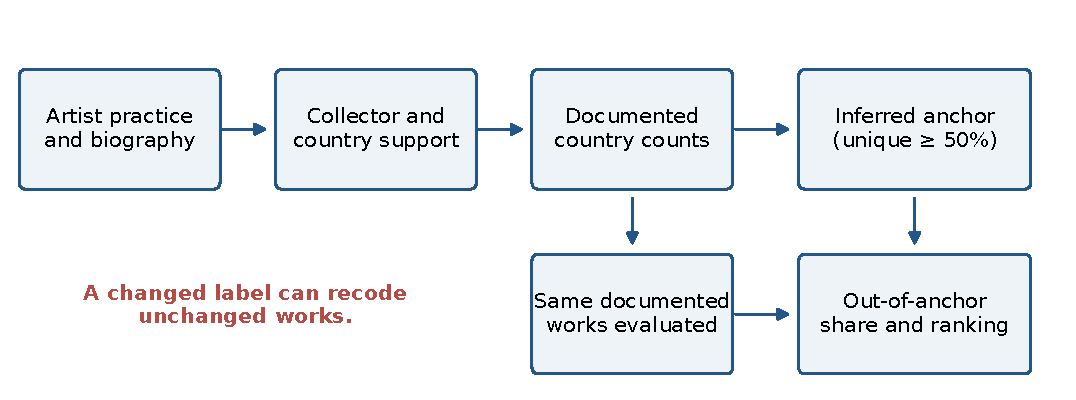
\includegraphics[width=\linewidth]{../figures/measurement_pipeline.pdf}
\caption{The measurement dependency. Collector and country support select documented counts. Those counts determine an anchor that is then used to classify the same works. Biographical evidence is a different input. A support-induced label change can recode an unchanged evaluation cohort.}
\Description{A left-to-right pipeline connects artist practice, documentation support, country counts, and an inferred anchor. Counts and the anchor feed an out-of-anchor share, illustrating reuse of documentation geography.}
\label{fig:pipeline}
\end{figure}

\section{Related Work and the Measurement Setting}
\subsection{Cultural geography and mediated visibility}
Street-art mapping already treats platforms as mediators. Honig and MacDowall map Melbourne street art through Instagram metadata \cite{honig2017}; their study motivates distinguishing an observed digital trace from the cultural practice generating it. Gomes reviews cultural mapping in relation to street art and intangible heritage \cite{gomes2025}. Project INDIGO develops systematic graffiti documentation \cite{indigo2022}. These works situate our analysis within an existing documentation agenda. We neither introduce cultural mapping nor treat a count of mapped works as a comprehensive measure of cultural value.

Nationality and residence also require separation in adjacent cultural-market research. Quemin examines nationality and location in contemporary-art recognition \cite{quemin2015}. Ferreira and Waldfogel study domestic music consumption using artist-origin information \cite{ferreira2013}. These are distinct domains and estimands, but they show why an origin variable is analytically consequential. An observed oeuvre concentration is useful for locating documented practice; using it as a proxy for an artist's biography requires a separate justification.

Volunteered geographic information research establishes spatial and contributor biases. Hecht and Stephens document urban bias across several platforms \cite{hecht2014}. B\'{e}gin and colleagues examine mapping behaviour as evidence about data quality \cite{begin2013}. Our collector deletions follow that established concern. The narrower question here is how a contributor's geographic contribution propagates through an artist-level label into destination comparisons. We analyze sensitivity, not contributor accuracy or motivation.

\subsection{Construct validity and outcome-derived labels}
Jacobs and Wallach explain how fairness depends on the relationship between a construct and its operationalization \cite{jacobs2021}. Selbst and colleagues warn against abstraction boundaries that omit the institutions and people shaping computational systems \cite{selbst2019}. These perspectives locate the relevant system boundary before the final dashboard: the artist definition, country support, documentation labour, and evidential status of the inferred label are part of the measurement system.

Reusing observations to construct and evaluate a variable is related to circular analysis \cite{circular2009}. Our concern is descriptive and semantic, rather than a claim that a particular significance test is invalid. No significance test is needed to show the domestic-share floor. Equally, the floor does not imply that every high domestic share is entirely artificial. Independent validation can support a proxy in a defined population, and observed concentration above the floor remains descriptive information. The issue is which inference the statistic licenses.

Data cascades \cite{cascades2021} and datasheets \cite{gebru2021} motivate carrying assumptions forward to downstream uses. We instantiate that principle with a computable support record: country panel, artist inclusion rule, source of the label, contributor-deletion outcomes, and a completion budget. This record accompanies a statistic rather than asserting that improved documentation alone validates an identity claim.

\section{Data, Units, and Analysis Design}
\subsection{A public export panel, not a global census}
On 14 October 2026 the public download page linked October CSV exports for Belgium (BE), Germany (DE), Spain (ES), the Netherlands (NL), Portugal (PT), and the United States (US). We retrieved all six, containing 48,690 markers, and recorded their URLs, byte sizes, and SHA-256 hashes. Four countries also had linked September exports: BE, ES, NL, and PT. The historical WIPO export is available on request \cite{sacwipo}; we did not obtain it. Our panel therefore audits a published rule on a later accessible dataset, and cannot validate or correct WIPO's 37-country numerical estimates.

Each row describes a platform marker, not necessarily a unique independently verified physical artwork. Marker IDs have no duplicates within the combined October panel, and each row's country field agrees with its export country. We do not conduct a coordinate-to-border validation. Multiple markers could still document the same artwork. Missing countries and uneven coverage within included countries remain unresolved.

The primary analysis retains markers declaring exactly one artist and providing a nonempty artist URL: 42,730 records and 12,373 distinct URLs. We use URLs rather than fuzzy name matching to define artist identity. This avoids inventing matches but does not prove that all URLs denote different people: aliases, collectives, and profile splits may remain. All statuses are included because the target is documented oeuvre geography, not the current stock of surviving murals. Active-only results are reported separately.

\begin{table}[t]
\caption{October export panel and primary cohort. ``Cohort'' counts works whose artist has a qualifying full-panel anchor. The last two columns use all primary single-artist records in each country, not only qualifying artists.}
\label{tab:data}\centering
\begin{tabular}{lrrrrr}\toprule
Country & Raw markers & Single artist & Cohort & Top collector (\%) & Nationality tag (\%)\\\midrule
BE & 8,208 & 7,080 & 5,305 & 17.4 & 26.2\\
DE & 9,571 & 8,176 & 6,003 & 13.5 & 7.4\\
ES & 11,539 & 10,360 & 7,798 & 10.9 & 4.1\\
NL & 4,308 & 3,740 & 2,713 & 9.8 & 11.7\\
PT & 3,847 & 3,550 & 2,725 & 41.8 & 29.5\\
US & 11,217 & 9,824 & 6,152 & 19.1 & 0.3\\\midrule
Total & 48,690 & 42,730 & 30,696 & --- & 10.3\\\bottomrule
\end{tabular}
\end{table}

\subsection{Labels, denominators, and conservative metadata comparison}
For artist $a$, let $n_{ac}$ be the number of retained markers in country $c$, and $n_a=\sum_c n_{ac}$. The anchor $h_a$ is defined when $n_a\geq3$, exactly one country attains the maximum count, and that maximum is at least $n_a/2$. Otherwise the procedure abstains. WIPO's published note does not specify a tie convention; our unique-maximum requirement is an explicit conservative implementation choice, not a claim about its unpublished code.

Let $A_0$ be artists assigned an anchor in the full October panel. This set contains 3,051 artists and 30,696 markers. Our primary country share is
\begin{equation}
 F_c(h)=\frac{\sum_{a\in A_0}n_{ac}\,\mathbf{1}\{h_a\ne c\}}{M_c},\qquad
 M_c=\sum_{a\in A_0}n_{ac}.
 \label{eq:share}
\end{equation}
We call it an \emph{out-of-anchor share}. Under a biographical interpretation of $h$, it might be presented as a foreign-artist share. Under its implemented definition, it measures how many documented works lie outside their artists' dominant documented countries. Country denominators remain fixed in the completion analysis; added documentation changes labels but never joins the evaluation cohort.

Nationality is stored in an artwork-level attribute, not a verified artist biography. We normalize a finite, released alias dictionary, parse JSON arrays when present, and accept only a recognized singleton value. We do not map regional identities such as Catalonia or Galician to a state, infer a country from an artist's name, or resolve ambiguous compound strings. For the artist-level comparison, at least one accepted tag is required; all substantive nonempty tags must be recognized singletons agreeing on the same value. Empty arrays count as missing. Nineteen artists have conflicting accepted singleton tags, and 26 have at least one ambiguous substantive tag; these exclusion categories can overlap. This conservative comparison yields 933 artists with both an anchor and consistent tags. It does not reproduce the 613 self-declared profiles used in WIPO's calibration.

\subsection{Support interventions and statistical interpretation}
Country-support analysis enumerates every nonempty subset of the six countries. On each subset we recompute anchors and classify every artist in $A_0$ as unchanged, reassigned, present but unassigned, or absent. The denominator is always 3,051 artists. An absent artist is not counted as a label reassignment. This distinction prevents a reduction in coverage from masquerading as an origin change.

For collector support we remove one recorded collector's markers at a time for each artist and recompute its anchor. Collector identity comes from the hunter URL. Eight primary records lack that field; they remain in artist totals but are not assigned to a synthetic collector for deletion. We report both any-deletion outcomes and deletion of each artist's largest collector. A deterministic URL ordering resolves equal-size collectors internally; identities are never published. The largest-collector control removes the same number of markers uniformly without replacement within each artist. Two hundred replicates use a fixed random seed. The comparator distinguishes structured geographic loss from loss of an equal amount of evidence; it is not a model of how collectors enter or leave the platform.

These analyses are finite-panel descriptions. Neither artists nor countries were probability-sampled. We therefore avoid population confidence intervals and significance tests for the panel statistics. The random-control quantiles describe Monte Carlo variation under the declared deletion mechanism. Completion envelopes describe possible allocations under an explicit budget. Neither is an interval for global street-art mobility. A local protocol was saved after inspecting schemas and country sizes but before computing these outcomes; it was not externally preregistered.

\section{Exact Completion Sensitivity}
\subsection{What the anchor guarantees and what it cannot identify}
For every assigned artist, $n_{a h_a}\geq n_a/2$. Summing over $A_0$ gives
\begin{equation}
 \frac{\sum_{a\in A_0} n_{a h_a}}{\sum_{a\in A_0} n_a}\geq\frac12.
 \label{eq:floor}
\end{equation}
The same lower bound holds for the mean of artist-level domestic fractions. It need not hold within each destination country: a receiving country can contain many works by artists anchored elsewhere. Nor does the bound cover works from unassigned artists. An analyst must specify both aggregation and inclusion before invoking it.

Equation~\ref{eq:floor} is a deterministic implication of the rule, not a discovery about artist behaviour. It also does not identify birthplace, nationality, or residence. Without restrictions linking those constructs to observed geography, the same count vector is compatible with different biographical origins. Independent biographical evidence or validated population-specific assumptions are needed. WIPO's calibration addresses a part of this problem; it does not make a six-country export panel equivalent to its historical coverage.

\subsection{Minimum documentation required for a target anchor}
Consider additional documented works belonging to existing artists. Let $x_{ac}\geq0$ be integer additions and $\sum_{a,c}x_{ac}\leq B$. A seventh category, OUT, represents any one previously unrepresented country. It suffices for our extrema because no evaluated work has an OUT destination. The additions are a sensitivity model for unobserved documentation: no such works are inserted into the source platform, and their existence is not asserted.

\begin{proposition}[Minimum target cost]
Under the unique-maximum, weak-majority, minimum-three rule, the least number of additions required to assign artist $a$ to target $c$ is
\begin{equation}
 q_a(c)=\max\left\{0,\;3-n_a,\;n_a-2n_{ac},\;
       \max_{d\ne c}n_{ad}-n_{ac}+1\right\}.
 \label{eq:cost}
\end{equation}
All additions can be placed in $c$. For strict majority, replace $n_a-2n_{ac}$ by $n_a-2n_{ac}+1$.
\end{proposition}
\begin{proof}
For any total of $x$ additions, placing all $x$ in $c$ maximizes the target count and weakly minimizes each rival count. Thus, if any allocation with that total qualifies, the all-target allocation qualifies. Under this allocation the three requirements are $n_a+x\geq3$, $2(n_{ac}+x)\geq n_a+x$, and $n_{ac}+x>\max_{d\ne c}n_{ad}$. Their integer lower bounds, together with $x\geq0$, give Equation~\ref{eq:cost}. The allocation attaining their maximum proves sufficiency.
\end{proof}

For example, counts $(3,2)$ require two additions to the second country to make it the unique anchor; one produces a tie. A unanimous three-work profile needs four additions in a previously unrepresented country. The cost describes the rule's sensitivity, not the number of actual works needed to establish nationality. A label can also become unresolved before it switches. If its leading count is $m$ and largest rival count is $r$, the cheapest tie costs $m-r$ additions, while eliminating weak majority costs $2m-n_a+1$. With at least two possible rival countries, additions can be distributed to attain the latter without creating another majority. Thus the minimum abstention cost is $\min\{m-r,2m-n_a+1\}$. The reference reporting routine checks both abstention and reassignment before stating that an anchor survives a budget.

\subsection{Sharp country envelopes under one shared budget}
For a fixed destination $c$, an artist contributes either $0$ or $n_{ac}$ to the foreign numerator. If $h_a=c$, the minimum cost to turn its contribution on is
\begin{equation}
 r_a^{+}(c)=\min_{d\ne c}q_a(d).
\end{equation}
If $h_a\ne c$, the minimum cost to turn the contribution off is $r_a^{-}(c)=q_a(c)$. Each change is one item with cost $r$ and value $n_{ac}$. Optimizing the numerator reduces to a 0--1 knapsack on artists. With $V_c^{+}(B)$ and $V_c^{-}(B)$ denoting its maximum values in the two directions, the exact extrema are
\begin{equation}
 F_c^{\min}(B)=F_c(h)-\frac{V_c^{-}(B)}{M_c},\qquad
 F_c^{\max}(B)=F_c(h)+\frac{V_c^{+}(B)}{M_c}.
 \label{eq:envelope}
\end{equation}

These bounds are sharp under the completion model: every selected item has a feasible all-target completion; distinct artists' completions add their costs without interfering. Conversely, any completion changing a contribution pays at least the corresponding minimum cost. We optimize over completions that retain a resolved anchor for every artist in $A_0$; abstaining completions do not define Equation~\ref{eq:share} and are excluded from these envelopes. The dynamic program uses $O(|A_0|B)$ time and $O(B)$ memory. Separate countries' endpoints can require different completions, so overlap of these envelopes alone does \emph{not} prove that a ranking can reverse.

\subsection{Joint country-ranking witnesses}
For destinations $c,d$, compare $F_c-F_d$ using the common integer denominator $M_cM_d$. An artist with target anchor $t$ has label-dependent contribution
\begin{equation}
 z_a(t)=-n_{ac}M_d\,\mathbf{1}\{t=c\}
       +n_{ad}M_c\,\mathbf{1}\{t=d\}.
\end{equation}
Relative to its baseline $h_a$, option $t$ has cost $q_a(t)$ and gain $z_a(t)-z_a(h_a)$. A multiple-choice knapsack selects at most one target for each artist. Each stage reads the previous stage's array, preventing incompatible targets from being selected together. We find the smallest budget whose maximum gain exceeds the integer amount needed for a strict reversal. This computes a single jointly feasible completion for each comparison rather than combining independent marginal extrema.

These calculations use standard dynamic programming. Their methodological value is the application-specific accounting: a single unobserved oeuvre change can recode many original works, and a destination comparison shares artists across its two numerators. Treating each marker or each country's uncertainty independently misses that dependency. Exhaustive small cases and independent mixed-integer programs check the implementation.

\section{Results}
\subsection{Anchors describe documented concentration}
The full panel assigns 3,051 of 12,373 artist URLs. Their 30,696 works contain 28,893 in their anchor country, giving a domestic fraction of 94.1\% and an out-of-anchor fraction of 5.9\%. Of the assigned artists, 653 have documented works in more than one panel country. This is strong observed concentration within the panel, but a concentration statistic is not an independently observed nationality share.

Under the conservative metadata comparison, 196 of 933 artists (21.0\%) have an anchor differing from their consistent nationality tag. Of these 196 disagreements, 172 (87.8\%) involve tagged countries outside the panel. This predominance identifies a practical mechanism: when an artist's recorded nationality is outside the available export support, a location-derived anchor can only place that artist inside the panel or abstain. We do not interpret a mismatch as a verified error or extrapolate its frequency to untagged artists.

The two variables also produce different activity summaries on an identical comparator cohort. For its 12,206 works, the anchor-based foreign count is 1,208 (9.9\%) and the tag-based count is 2,473 (20.3\%). Propagating an artist's consistent tag to untagged works adds an assumption, so we also compare only records with their own accepted singleton tag. On those 3,461 records with assigned anchors, the counts are 359 (10.4\%) and 715 (20.7\%), respectively. This second comparison uses no tag propagation. It still relies on unverified metadata and is selected by tag availability.

Tag coverage itself is uneven: only 27 of 9,824 primary US records have a nonempty tag, compared with 1,047 of 3,550 Portuguese records. A complete-case comparison is therefore not a representative validation sample. It establishes a material difference between two available operationalizations and the need to retain their evidential status.

\subsection{Country support changes availability and attribution}
Figure~\ref{fig:support} summarizes all country subsets. Removing one country yields 20--30 reassigned anchors, 53--150 present-but-unassigned artists, and 155--655 absent artists, depending on the omitted country. The reassignment counts are modest relative to the full cohort; disappearance is the larger consequence. Both matter, but they answer different questions.

For single-country support, assigned labels can only name that country. Among the original cohort, 12--37 artists are reassigned, 108--208 are present but unassigned, and 2,141--2,658 are absent. Conditional on being assigned in a single-country export, every documented work is domestic by definition. That is a statement about measurement support, not evidence that the city's artists never work elsewhere.

A coverage-aware report therefore needs at least three quantities: how much of the original population remains represented, how much remains assignable, and how many retained artists change labels. Reporting only a high agreement rate among surviving assigned artists would suppress the largest support effects.

\begin{figure}[htbp]
\centering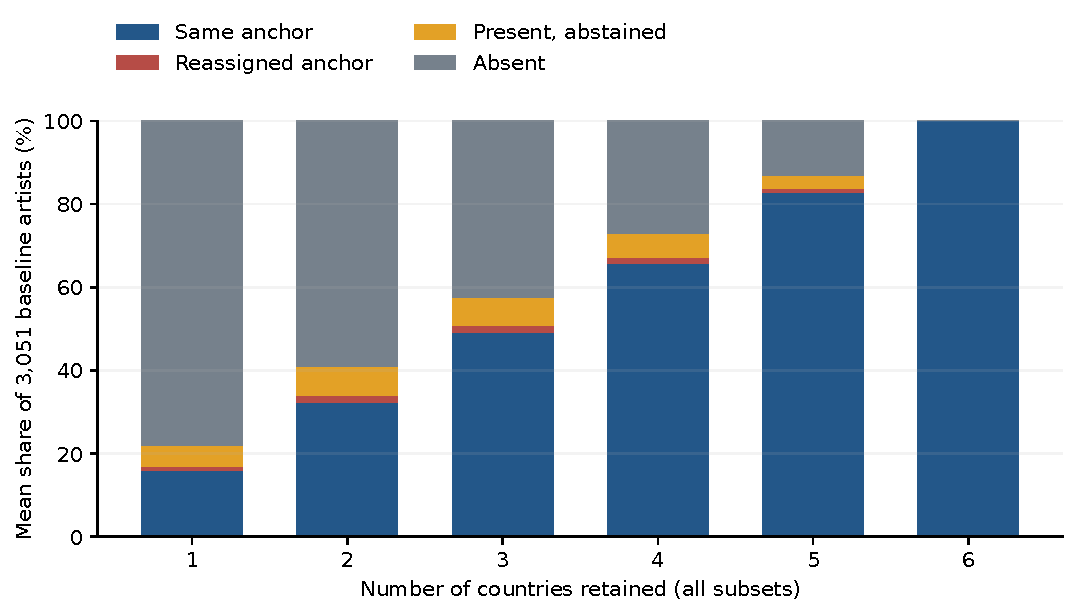
\includegraphics[width=.95\linewidth]{../figures/country_support.pdf}
\caption{Country-support outcomes averaged across all subsets of each size. The denominator always includes all 3,051 full-panel assigned artists. The figure separates disappearance from abstention and reassignment; a smaller export support need not imply a large reassignment rate among the artists it retains.}
\Description{A stacked bar plot shows increasing same-anchor retention as one to six countries are retained, with absent artists forming the largest category at small support sizes.}
\label{fig:support}
\end{figure}

\subsection{Collector concentration has structured influence}
Across all one-collector deletions, 1,035 artists (33.9\%) retain their original anchor in every deletion, 45 (1.5\%) have at least one reassignment, and 1,988 (65.2\%) have at least one abstention. Reassignment and abstention categories can overlap. Most fragility is lost assignability, not a different country label.

Deleting each artist's largest collector yields 38 reassignments, 1,948 abstentions, and 1,065 unchanged anchors. Equal-size random marker deletion produces a mean of 8.5 reassignments, with a central 95\% Monte Carlo range of 3--14 across 200 replicates (Figure~\ref{fig:collector}). Its mean abstention count is 1,924.3, with a corresponding range of 1,917--1,931. Thus, structured collector loss particularly affects the direction of resolved labels, while much of the abstention is explained by how many records remain.

The result is not driven only by three-work profiles. Among 748 assigned artists with at least ten works and at least two identified collectors, 23 admit a reassignment under some collector deletion and 113 admit an abstention; 618 retain the same anchor under every deletion. Deleting the largest collector in this subgroup reassigns 18 and makes 101 unassigned. These are sensitivity observations, not evidence that collectors are unreliable. A prolific local collector may document an artist accurately while still supplying a geographically concentrated slice of that artist's career.

\begin{figure}[htbp]
\centering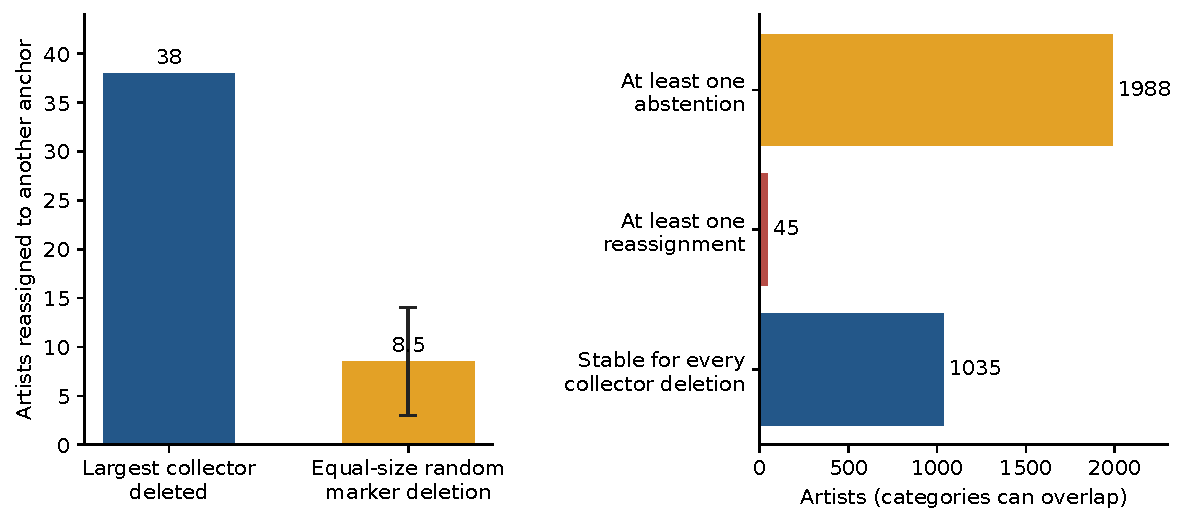
\includegraphics[width=.97\linewidth]{../figures/collector_influence.pdf}
\caption{Collector influence. Left: deleting the largest collector per artist produces 38 resolved anchor changes; deleting the same number of random records produces a mean of 8.5. The error bar is the central 95\% range across 200 random mechanisms, not a population confidence interval. Right: any-deletion outcomes; reassignment and abstention may overlap.}
\Description{Two plots compare 38 structured reassignments with about 8.5 random reassignments and show 1,035 always-stable artists, 45 with any reassignment, and 1,988 with any abstention.}
\label{fig:collector}
\end{figure}

\subsection{Small shared budgets can change destination comparisons}
Baseline destination out-of-anchor shares range from 3.5\% in Spain to 11.5\% in the Netherlands. Equation~\ref{eq:envelope} yields the sharp envelopes in Figure~\ref{fig:completion}. With 306 additions, approximately 1\% of the 30,696-work evaluation cohort, the Netherlands' share ranges from 6.1\% to 24.9\%; Portugal's ranges from 3.9\% to 21.2\%. With 1,534 additions, approximately 5\%, the ranges widen to 1.4--69.5\% and 0.4--65.3\%, respectively. Every endpoint keeps the original works and country denominators unchanged.

The budget is shared across all artists, not allocated independently to every artist or every destination. Nonetheless, each country's displayed endpoint optimizes a different possible completion. The numerical width should not be read as a likely error bar. An unconstrained worst-case allocation may be substantively implausible; its purpose is to expose what the geographic data alone do not rule out. Additional evidence can restrict which artists and target countries are plausible.

\begin{figure}[htbp]
\centering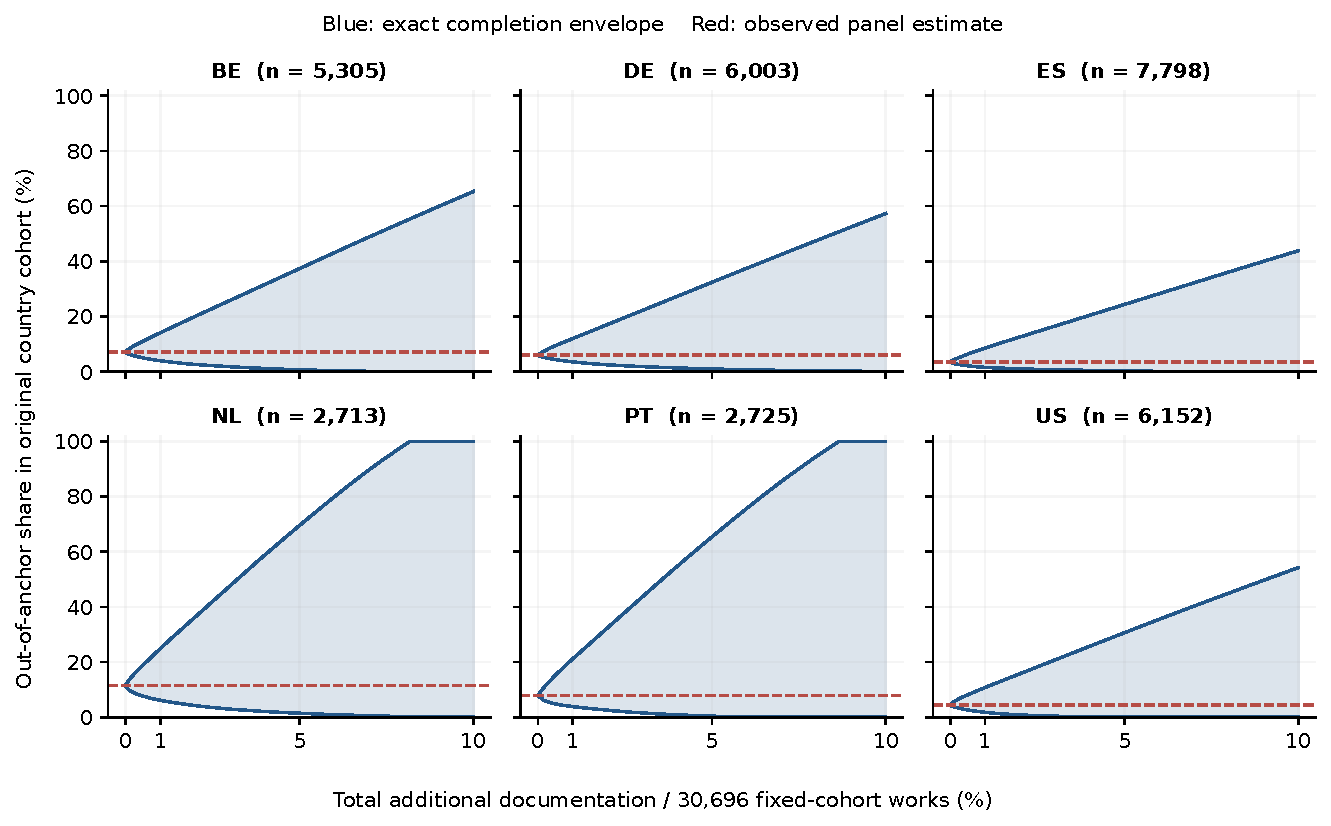
\includegraphics[width=\linewidth]{../figures/completion_envelopes.pdf}
\caption{Exact fixed-cohort completion envelopes. The horizontal budget is global and permits additional documentation for existing assigned artists in any country. No additional work enters the evaluated cohort. Country-specific extrema may use different allocations and are conditional sensitivity bounds, not estimated unseen activity.}
\Description{Six small multiples display baseline out-of-anchor shares as dashed lines and expanding sharp lower and upper envelopes as the global addition budget increases to ten percent.}
\label{fig:completion}
\end{figure}

Joint optimization strengthens the result beyond marginal overlap. Portugal initially exceeds Belgium by 0.802 percentage points; 14 jointly allocated additions suffice for a strict reversal, and no smaller budget does. The Netherlands initially exceeds Portugal by 3.573 points; the minimum is 62. The largest gap, Netherlands--Spain at 7.975 points, needs 352 additions. Figure~\ref{fig:ranks} reports all 15 pairwise minima. Fourteen comparisons can be reversed within a global budget of 306, while the remaining pair requires 352. This does not imply that one completion reverses all 15 pairs simultaneously: every pair is optimized separately.

A concrete minimum-budget witness changes five artists' documented anchors (Table~\ref{tab:witness}). It changes Belgium's foreign numerator from 376 to 396 and Portugal's from 215 to 203, while their denominators remain 5,305 and 2,725. Their shares become 7.465\% and 7.450\%, respectively. The narrowly reversed ordering demonstrates sensitivity without asserting that the counterfactual works exist.

\begin{table}[t]
\caption{One jointly feasible, minimum-budget Portugal--Belgium reversal. Counts are observed; additions are counterfactual. Anonymous row labels identify no artist. Unlisted country counts are zero.}
\label{tab:witness}\centering
\begin{tabular}{llccc}\toprule
Profile & Observed counts & Initial anchor & Target & Additions\\\midrule
A & BE:4, ES:1, NL:3 & BE & NL & 2\\
B & BE:16, DE:2, ES:12 & BE & ES & 6\\
C & ES:7, PT:6 & ES & PT & 2\\
D & ES:1, PT:3, US:4 & US & PT & 2\\
E & PT:3, US:4 & US & PT & 2\\\midrule
Total & & & & 14\\\bottomrule
\end{tabular}
\end{table}

\begin{figure}[htbp]
\centering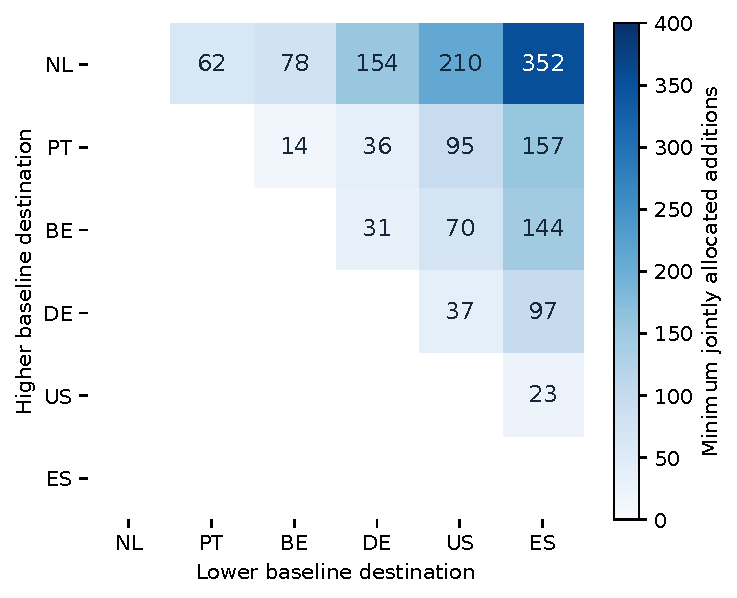
\includegraphics[width=.8\linewidth]{../figures/rank_reversal.pdf}
\caption{Smallest global addition budget for each strict destination-order reversal. Rows are higher baseline destinations; columns are lower baseline destinations. Each cell uses a single joint completion satisfying both country numerators. Cells are separate counterfactuals, not one common reversal scenario.}
\Description{An upper triangular matrix shows minimum addition counts from 14 to 352 for reversing each ordered pair of six destinations.}
\label{fig:ranks}
\end{figure}

\subsection{Temporal stability does not supply biographical validation}
The four-country September panel contains 27,250 raw markers and its October counterpart 27,902. There are 663 new marker IDs and 11 no longer present. Among 1,722 previously assigned artists, none changes to another resolved anchor and seven become unassigned. On 18,078 common records with unchanged artist URL and country and a previously assigned artist, none changes a resolved domestic/out-of-anchor classification; 14 become unresolved.

This is a useful negative result. The dataset does not exhibit an observed month-to-month wave of attribution changes in this window. The completion experiments therefore remain sensitivity experiments, not descriptions of the month's actual evolution. Short-term persistence of a label also cannot establish that it denotes nationality.

New uploads are not new production. Of 603 newly documented primary single-artist markers, 221 have parseable creation-date attributes and 149 of those predate September 2026. Missing and inaccurate creation dates remain possible. The result cautions against interpreting changes in platform counts as contemporaneous artist travel or cultural growth.

\subsection{Alternative inclusion rules and computational verification}
The concentration finding persists under the inclusion variants in Table~\ref{tab:sensitivity}. Active-only, strict-majority, and minimum-ten analyses change which artists qualify and therefore have distinct denominators. The collaboration extension counts each recorded marker--artist URL pair once. It is not an artwork-weighted statistic: collaborators can contribute multiple edges, and 353 markers declare more than the four artist-link columns available in the export. This extension is incomplete and is reported as a sensitivity check only.

\begin{table}[t]
\caption{Inclusion sensitivities. Domestic percentages refer to each variant's own assigned cohort, so their differences are not causal effects.}
\label{tab:sensitivity}\centering
\begin{tabular}{lrrr}\toprule
Rule & Assigned artists & Cohort records/edges & Domestic (\%)\\\midrule
Primary: all statuses, $n\geq3$ & 3,051 & 30,696 & 94.1\\
Active markers only & 2,742 & 26,533 & 94.3\\
Strict majority & 3,003 & 30,298 & 94.7\\
At least ten markers & 841 & 20,300 & 93.7\\
All available artist links & 3,918 & 39,930 & 94.0\\\bottomrule
\end{tabular}
\end{table}

An independent Counter-based implementation agrees on all 3,051 primary anchors and the domestic numerator. Exhaustive enumeration verifies Equation~\ref{eq:cost} on 384 count-vector/target/rule cases, including arbitrary distributions of additions; 200 random eight-item knapsack instances agree at every budget with exhaustive subset search. Exhaustive cases also verify the minimum abstention cost. A small joint cohort checks the country envelopes directly. Independent mixed-integer optimization verifies all twelve country extrema at budget 306 and four joint-ranking minima, including both the smallest and largest observed minima. All sixteen optimizations reach certified optimal status. The released source retains these checks and exact environment versions.

\section{A Reporting Discipline for Cultural Platforms}
\subsection{Separate evidence about people from evidence about records}
The useful output of this audit is not a corrected nationality for every artist. It is a separation of evidential objects. An artist record should store a biographical attribute with its source and verification status independently from an oeuvre anchor computed over a named panel and date. A dashboard should expose the latter as \emph{documented anchor}, with at least the counts, eligibility rule, and export support needed to reproduce it. Unknown biographical origin remains unknown even when the anchor is computationally stable.

Curators can use documented practice to find artists active in a place, and researchers can study concentration around an indexed scene. Citizenship, heritage, birthplace, and present residence need separate evidence, with support for correction and multiple affiliations.

\subsection{Attach decision-specific support evidence}
Our reference implementation computes anchors, collector-deletion states, completion costs, country envelopes, and joint ranking minima from a frozen CSV panel. A separate JSON reporting routine preserves supplied biographical evidence and its source independently; it never fills that field from geography. A platform integrating these routines can report the support condition under which an ordering remains fixed. For example, the observed Portugal--Belgium ordering is not stable under the declared unrestricted completion model once the total budget reaches 14. That is an actionable statement about the displayed comparison; it does not assign either country a true position in global mobility.

The budget must be supplied or justified by the application, not silently learned from the same incomplete platform counts. If plausibility rules exclude certain artist--country pairs, the target-cost options can be restricted accordingly. The algorithm will then describe that narrower model. A certificate is only as informative as the admitted additions, artist identity, and fixed evaluation cohort. Publishing the restrictions allows readers to contest the assumption rather than merely the numeric ranking.

A dashboard can report coverage and unordered country comparisons when its displayed ranking is unstable under a justified budget. This is a reporting choice, not a claim of equal cultural value; its effect on decision quality remains untested.

\subsection{Institutional and commercial implications}
Municipal dashboards and commissioning directories supply a plausible deployment setting. The contribution could support a data-quality component that audits cultural indicators before they are reused in procurement, tourism analytics, or research. Its outputs are uncertainty and provenance records rather than an automated eligibility score. The platform's existing partner products demonstrate such an institutional market; we have not measured demand, willingness to pay, procurement outcomes, or a startup's commercial viability.

A responsible implementation should fund artist-controlled correction and retain the labour and context behind documentation. Collector concentration is not a defect to be remedied by deleting contributions: it can reflect valuable expertise and sustained local effort. The audit instead helps distinguish contributions that enrich a map from evidence sufficient to support a biographical claim.

Commercial use of the source data requires appropriate permission. The public open-data page permits academic analysis and restricts non-academic integration and redistribution \cite{sacdata}. Releasing general-purpose source code does not transfer rights to the underlying records or images. We publish aggregate analysis and retrieval instructions, not artwork imagery, precise coordinates, collector identities, or a mirror of the dataset. No patentability or exclusive technical novelty is asserted.

\section{Limitations and Implications for Further Research}
Artist URLs are platform identities. Duplicate physical works, split profiles, collectives, transcriptions, and inaccurate attribution can affect all statistics. We do not correct these through language-model inference or artist-name geocoding. Single-artist analysis avoids ambiguous attribution weights but excludes collaborations; the multi-link sensitivity does not recover artists beyond the available columns.

Nationality tags are sparse, culturally and administratively imperfect, and potentially supplied by the same contributors who document location. They are neither independent ground truth nor an ethically sufficient basis for nationality-based eligibility. Their role here is to show that two stored quantities disagree even on a conservative common cohort. Independent artist-confirmed biographies could assess validity, subject to appropriate governance and permissions.

The completion model allows unobserved documentation in any country for existing assigned artists. Its budgets are analytic scenarios, not estimates of missing works. It excludes new artists, changes to identity, corrections to original marker countries, and artwork-level duplication. Adding works for currently unassigned artists could change both the cohort and the denominator; that is a different estimand. Our fixed-cohort construction deliberately isolates recoding. A feasible arithmetic completion is not proof that those artworks exist or that travel is practical.

Collector deletions are stress tests. They do not simulate a random sample of independently disappearing volunteers, and hunter URLs do not capture every editor who helped produce a record. The random controls quantify one matched mechanism rather than test a universal hypothesis. Four-country temporal replay covers one monthly interval and finds no resolved switches; it does not establish long-term stability.

The study documents a pathway to misinterpretation, not observed discrimination, income loss, or incorrect public funding. Independent origins, commissioning practices, broader panels, and restricted completion models would permit stronger evaluations. The present contribution keeps those missing observations distinct from what the available records establish.

\section{Conclusion}
A country of documented practice is useful cultural information, but it is not automatically an artist's origin. In a six-country street-art export panel, the published geography-derived rule produces highly local-looking activity while disagreeing with consistent nationality metadata for one fifth of comparable artists. Collector and country support affect which artists remain represented and assignable; exact shared-budget calculations show that some destination orderings can reverse through a small amount of additional documentation. A monthly replay exhibits no resolved label changes, keeping the sensitivity findings distinct from observed change. The practical contribution is a reproducible way to preserve those distinctions: label documented anchors explicitly, retain biographical provenance separately, and qualify destination comparisons with their support assumptions.

\clearpage
\section*{Ethical Considerations and Adverse Impacts}
The analysis follows the platform's academic-use conditions and publishes aggregate findings without precise coordinates, imagery, collector names, or individual nationality judgments. Sensitivity to a collector's contribution is not an allegation about that collector's integrity. Origin proxies and nationality metadata should not determine citizenship, belonging, or access to cultural support without separate justification and a correction process. The completion code can expose weak rankings; it should not be used to manufacture records or impersonate contributors. The reported counterfactuals are computed locally and do not modify the platform.

\section*{Generative AI Usage Statement}
GPT-6 through Codex assisted research design, literature review, code, analysis, figures, and manuscript drafting. The author retains responsibility for the work.

\clearpage
\bibliographystyle{ACM-Reference-Format}
\bibliography{references}
